\chapter{Implementation}
\section{Architecture}
We implemented the algorithm as a new filter in the Insight Segmentation and Registration Toolkit (ITK).  The ITK toolkit is a collection of image processing and statistical analysis algorithms for biomedical imaging applications.  Additionally, the ITK toolkit is open-source software, which allows other researchers to learn directly how this system was implemented and make improvements in the future.  Including the algorithm in the ITK toolkit makes it available to a large existing research community.  Additionally, we created a GUI module for the 3D Slicer medical visualization program that provides easy access to the algorithm via an intuitive visual interface.  We also created a command line interface to the ITK filter that can be used to process large numbers of data sets in a batch mode.  Choosing to implement the algorithm as an extension of already established tools facilitates adoption of the algorithm in clinical studies.

The stochastic tractography algorithm is a Monte Carlo algorithm which samples the high dimensional parameter space of fiber tracts.  This parameter space is large because fiber tract are characterized by a sequence of segment orientations, each of which can be considered a separate parameter describing the fiber tract.  As such, it may take many samples to accurately approximate the posterior distribution of these parameters.  However, since these samples are IID, the samples can be generated in parallel.  Implementing the system in a multithreaded fashion enables parallel sampling of the tract distribution.

ITK  provides a framework for implementing multithreaded algorithms.  The ITK multithreading framework assumes that the output region can be divided into disjoint sections with each thread working exclusively on their own section of the output image.  This design prevents threads from simultaneously writing to the same memory region, which may cause unexpected results.  However, since the stochastic tractography algorithm generates tracts that may span the entire output image, dividing the output region into disjoint sections is not possible.  Additionally, in order to obtain statistics on these tracts, we need to output the generated tracts as well as the resultant connectivity image.  Thus the existing ITK framework for implementing multithreaded filters is not very useful for our stochastic tractography filter.  Fortunately ITK also provides basic multithreading functions which allowed us to create a custom multithreaded design for the stochastic tractography system that is still within the ITK framework. 

\begin{figure}[t]
  \center
	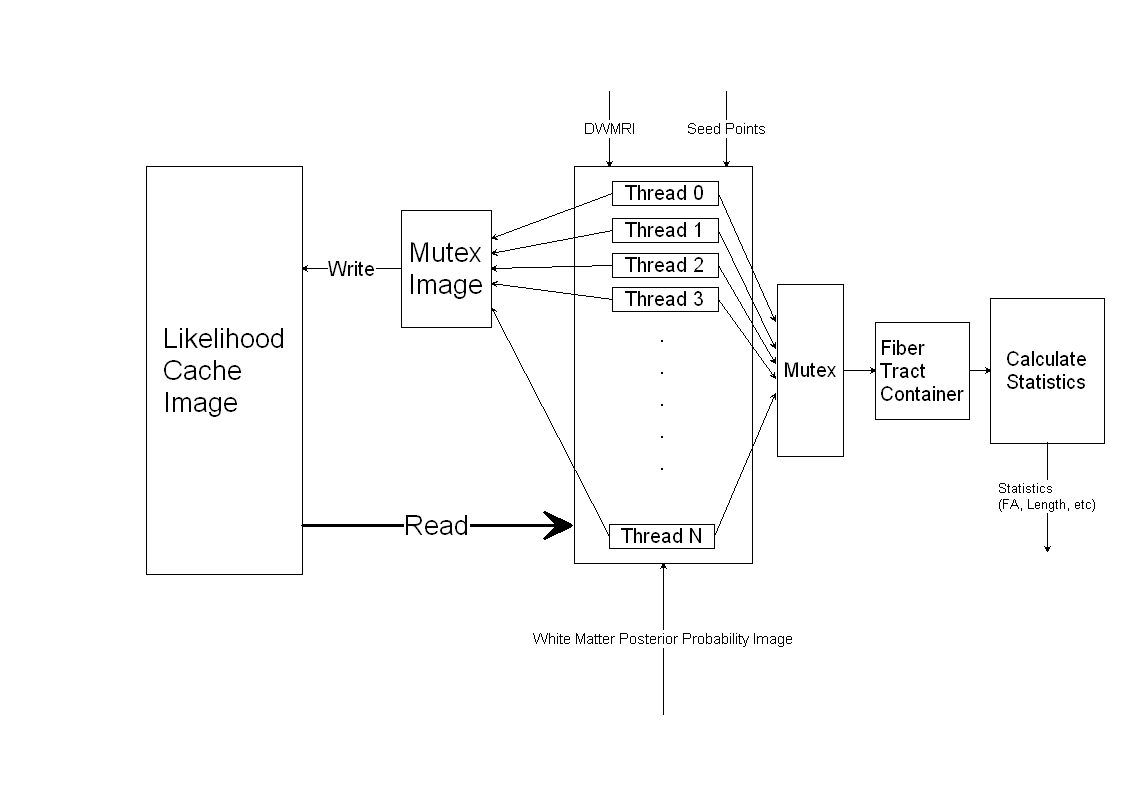
\includegraphics[width=\linewidth]{filterblock}
	\caption{A block diagram of the filter showing its shared likelihood cache and multithreaded architecture.}
	\label{fig:filterblock}
\end{figure}

Each thread of stochastic tractography filter is an instance of the stochastic tractography algorithm. The block diagram in figure \ref{fig:filterblock} demonstrates graphically the architecture of the ITK stochastic tractography filter.  Every thread allocates it own independent memory for the tract that it is currently generating.  Once the tract has terminated, the thread stores a memory pointer to the completed tract in a tract pointer container that is shared among all threads.  The tract pointer container is protected by a mutex, which serializes write operations so that only one thread can store its completed tract in the vector at a time.  Once the filter has generated enough samples, the tracts can be transferred to an output image to create a connectivity map.  Additionally other statistics can be computed on the tracts.  In essence, we divide the process into two sections, a multithreaded portion that samples the tracts and a single threaded portion which accumulates the tracts and calculates relevant statistics on them.

The most computationally expensive part of the algorithm is the calculation of the likelihood distribution.  The algorithm must compute probabilities for 2,562 possible fiber orientations in a voxel.  Fortunately, this likelihood distribution is a deterministic function of the diffusion observations within that voxel.  The filter runs much faster, at the cost of additional memory, by caching the generated likelihood distribution for later access.  Caching is effective because in highly anisotropic regions of the brain, the sampled tracts are expected to be dense causing many of the sampled tracts to visit the same voxels many times.

The cache is implemented as an image whose voxels are re-sizable arrays.  ITK's optimized pixel access capabilities enable quick access to the likelihood distribution associated with any voxel in the image.  On creation, every voxel in the likelihood cache image is initiated to a zero length array.  Whenever the algorithm encounters a voxel, it first checks to see if the likelihood cache contains this voxel by testing if associated array is zero length.  If the voxel has never been visited, the associated array is resized and the computation of the likelihood distribution associated with this voxel is stored inside the newly resized array.

Using a shared likelihood cache between multiple concurrent threads creates additional complexities.  Simultaneous writes to the cache would cause unexpected behavior.  Additionally there is the possibility of one thread reading an incomplete cache entry while another thread is trying to write it.  One possible solution is to ensure that only one thread can read or write to the likelihood cache at a time.  This is easily implemented by serializing access to the likelihood cache using a mutex.  A mutex serves as a lock on data.  A thread will wait to obtain a lock on the data before it proceeds to the next section of code.  Inside this section, which is called the critical section, the thread holds the lock ensuring exclusive access to the otherwise shared data.  All other threads must wait and idle while the thread which owns the lock finishes it operations.  Since threads must access the likelihood cache very often, this results in a situation where many threads are waiting for other threads to finish accessing the likelihood cache.  The serialized access to the likelihood cache creates a bottleneck, which in the worse case would result in performance that is only marginally better than a single threaded version of the filter.
\begin{figure}
  \center
  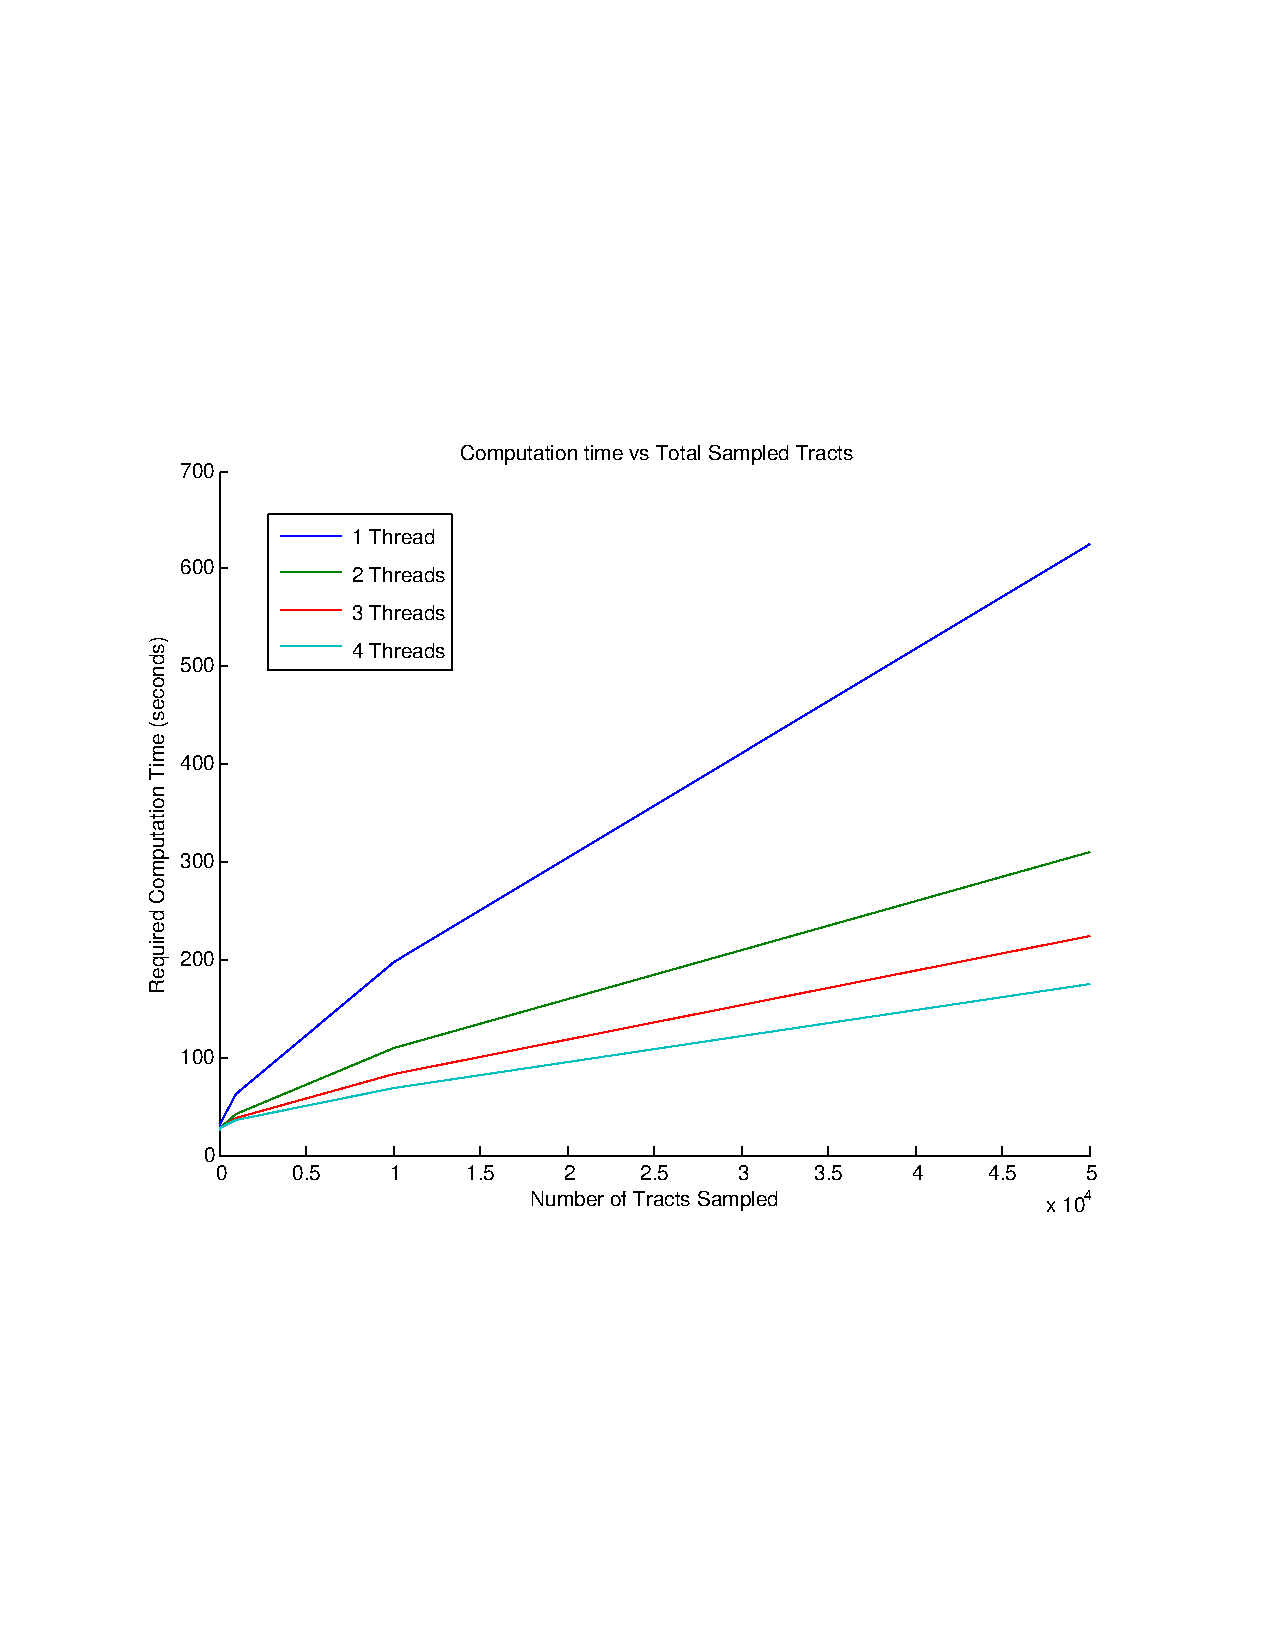
\includegraphics[trim = 20mm 70mm 20mm 70mm, clip, width=0.75\linewidth]
	  {timepertracts}
	\caption{A graph displaying the amount of time needed to sample a number of tracts.  Each line represents the algorithm's performance using different numbers of threads.  This test was run on a 4 processor machine.}
	\label{fig:performance}
\end{figure}

Access collisions to the likelihood cache can be reduced if we increase the granularity of the lock.  Instead of using one large lock for the entire likelihood cache image, we use a lock for each voxel.  The probability of two threads accessing the same voxel simultaneously is much less than the probability of two threads accessing any part of the likelihood cache.  These per voxel locks are conveniently constructed using an ITK image whose voxel data type is a mutex.  Similar to the likelihood cache, this collection of mutexes is indexed by coordinates which correspond to the coordinates of the voxels in the DWI input data.  Again, access to the mutex image is fast due to ITK's optimized access operators for data types indexed by coordinates.  The only cost to using this high resolution mutex image is the additional memory required to store pixel mutexes.  However this cost is small since a mutex is essentially a Boolean variable.  The mutex image allows different voxels in the likelihood cache image to be updated simultaneously, increasing the rate that the likelihood cache is filled.  The advantage of using a mutex image is most evident when tracking in highly isotropic regions,  where collisions are very unlikely to occur, since the sampled paths are very dispersed.  Even on uni-processor systems, using multiple threads may improve performance since the rate of encountering an unvisited voxel may be higher, thus filling the likelihood cache faster. Figure \ref{fig:performance} demonstrates the required computation time for a given number of tracts under different number of threads.

Additionally, to compute the weighted least squares estimates for the log tensor model parameters, we must first estimate the weights.  These weights are found by calculating a least squares estimate of the true intensities of each voxel.  The $\mathbf{A}$ matrix \ref{eq:fulllogtensor} used in this least squares estimation is a function solely of the magnetic gradient directions and associated b-values, which are the same for every voxel in the image.  Since the same $\mathbf{A}$ matrix is used for each voxel in the least squares calculation, a common optimization is to orthogonalize the $\mathbf{A}$ matrix by computing its QR decomposition.  While this operation is computationally expensive, it is performed only once for the entire DWI image.  The orthogonalized $\mathbf{A}$ matrix reduces the cost of computing the weights for every voxel.

\section{ITK Stochastic Tractography Filter}
The Stochastic Tractography Filter is implemented as a multithreaded image filter in ITK under the class name itk::StochasticTractographyFilter.  The filter is templated over the DWI and white matter probability map input image types and also on the connectivity map image type.  The filter expects the DWI input image type to be an ITK VectorImage Type.  The code below demonstrates how to instantiate the Stochastic Tractography Filter.
\begin{verbatim}
  //Define Types
  typedef itk::VectorImage< unsigned short int, 3 > DWIVectorImageType;
  typedef itk::Image< float, 3 > WMPImageType;
  typedef itk::Image< unsigned int, 3 > CImageType;
  typedef itk::StochasticTractographyFilter< DWIVectorImageType, WMPImageType,
    CImageType > PTFilterType;
  //Allocate Filter
  PTFilterType::Pointer ptfilterPtr = PTFilterType::New();
\end{verbatim}

The filter's required inputs and parameters must be set before it can be run.  Table \ref{tab:filterinputs} lists filter methods that should be called to set the required inputs and parameters,  and a short description of what each methods expects as arguments.

\begin{table}
  \center
  \begin{tabular}{| l | p{8cm} |}
    \hline 
    \textbf{Filter Member Method} & \textbf{Description}\\
    \hline
    \small{SetInput} & DWI Image: An ITK VectorImage consisting of a vector of DWI measurements including the baseline b0 measurements, at each voxel. \\
    \hline
    \small{SetWhiteMatterProbabilityImageInput} & White Matter Probability Input: An ITK image whose voxel values range from 0 and 1 representing the posterior probability that the voxel is a white matter.  \\
    \hline
    \small{SetbValues} &  b-Values: An ITK VectorContainer whose elements are the corresponding b-values for the DWI input image.  The b0 measurements must have a 0 b-value. \\
    \hline
    \small{SetGradients} & magnetic gradient directions: An ITK VectorContainer whose elements are 3 dimensional vnl vectors.  These vectors should be unit length.\\
    \hline
    \small{SetMeasurementFrame} & DWI Measurement Frame: A 3x3 vnl matrix which transforms the gradient directions to the physical reference frame of the image.  For instance multiplying a magnetic gradient direction vector by the Measurement Frame Matrix will take the vector to the RAS reference frame if RAS is the physical frame of the DWI image. \\
    \hline
    \small{SetMaxTractLength} & Maximum Tract Length: A positive integer that sets the maximum length of a sampled tract.  This can also be interpreted as the number of segments which comprise the tract when using the default step size of 1 unit in the physical frame of the DWI image. \\
    \hline
    \small{SetTotalTracts} & Total Sampled Tracts: A positive integer that sets the total number tracts to sample from the seed voxel. \\
    \hline
    \small{SetMaxLikelihoodCachSize} & Maximum Likelihood Cache Size(MB) A positive integer that sets the maximum size of the Likelihood Cache in megabytes.\\
    \hline
    \small{SetSeedIndex} & Seed Voxel Index:  The discrete index of the seed voxel, in the (IJK) reference frame of the image to start tractography.\\
    \hline
  \end{tabular}
  \caption{ITK Stochastic Tractography Filter Required Inputs and Parameters}
  \label{tab:filterinputs}
\end{table}

The code below is a continuation of the demonstration above and shows how to setup the filter's required inputs and parameters.  The inputs to these methods are provided by ITK's image readers.
\begin{verbatim}
  ptfilterPtr->SetInput( dwireaderPtr->GetOutput() );
  ptfilterPtr->SetWhiteMatterProbabilityImageInput( wmpreader->GetOutput() );
  ptfilterPtr->SetbValues(bValuesPtr);
  ptfilterPtr->SetGradients( gradientsPtr );
  ptfilterPtr->SetMeasurementFrame( measurement_frame );
  ptfilterPtr->SetMaxTractLength( maxtractlength );
  ptfilterPtr->SetTotalTracts( totaltracts );
  ptfilterPtr->SetMaxLikelihoodCacheSize( maxlikelihoodcachesize );
  ptfilterPtr->SetSeedIndex( seedindex );
\end{verbatim}

The filter can then be run by calling the Update method.
\begin{verbatim}
  ptfilterPtr->Update();
\end{verbatim}

For the specified seed voxel, the filter outputs a connectivity map and a container holding all of the sampled tracts used to generate the connectivity map.  The container of sampled tracts can be further processed outside of the stochastic tractography filter to obtain various statistic on the sampled tracts.  Additional seed voxels can be included in the seed region by changing the seed voxel index and rerunning the filter.  The statistics for a multi-voxel seed region can be analyzed by accumulating statistics for all seed voxels within the seed region.  These outputs can be accessed by calling the  \texttt{GetOutput} and  \texttt{GetOutputTractContainer} methods after calling the  \texttt{Update} method.  The code below continues the example above and demonstrates how to obtain the filter's outputs.
\begin{verbatim}
  PTFilterType::TractContainerType::Pointer tractcontainer = 
    ptfilterPtr->GetOutputTractContainer();
  CImageType::Pointer cmap = ptfilterPtr->GetOutput();
\end{verbatim}

\section{Command Line Module Interface}
The command line module interface provides an easy to use method of performing common tasks which use the ITK stochastic tractography filter.  The command line module takes as input a DWI volume, a white matter probability map and a label map to produce a connectivity probability map and fractional anisotropy and length statistics for a selected seed region in the label map.  Currently the command line module is designed to work only with NRRD formatted volumes due to its support of the diffusion measurement frame, but future revisions of the software will extend support to other formats.

The command line module is named \texttt{StochasticTractographyFilter}.  Calling the executable with the \texttt{--help} flag will list all available inputs and options as well as a short description of each item (Appendix B).  This section will demonstrate two typical usages of the command line module interface.

Given a DWI volume, an associated white matter probability map and a label map, the command line module can be used to generate an image that provides the probability of connectivity from an ROI in the label map to all other voxels in the DWI.  The label map is an integer valued image that segments voxels into different classes or labels.

Let \texttt{case24} be the name of the subject we are interested in analyzing.  The directory \texttt{case24} contains all relevant files for that subject.  It will also hold the output files generated by the command line module.  Before executing the command line module interface, a possible list of files in the \texttt{case24} directory may include:
\begin{verbatim}
  case24_DWI.nhdr (DWI NRRD header)
  case24_DWI.raw (DWI NRRD data)
  case24_whitematterPB.nhdr (White Matter Probability Map NRRD header)
  case24_whitematterPB.raw (White Matter Probability Map NRRD data)
  case24_labelmap.nhdr (Label Map NRRD data)
  case24_labelmap.raw (Label Map NRRD data)
\end{verbatim}
Assuming that the starting ROI is labeled $15$ inside the labelmap, the stochastic tractography filter can be run by executing the command below within the \texttt{case24} directory: 
To run the command line module, execute the command:
\begin{verbatim}
  StochasticTractographyFilter -c 6500 -m 500 -t 200 -e 15 -l 15
  -r -o case24_RUN0 case24_DWI.nhdr case24_whitematterPB.nhdr
  case24_labelmap.nhdr
\end{verbatim}
After the command completes, the \texttt{case24} directory will contain the following additional files:
\begin{verbatim}
  case24_RUN0_CMAP.nhdr (Connectivity Map NRRD header)
  case24_RUN0_CMAP.raw (Connectivity Map NRRD data)
  case24_RUN0_TENSOR.nhdr (Tensor image NRRD header)
  case24_RUN0_TENSOR.raw (Tensor image NRRD data)
  case24_RUN0_COND.nhdr (Conditioned Connectivity Map NRRD header)
  case24_RUN0_COND.raw (Conditioned Connectivity Map NRRD data)
  case24_RUN0_CONDFAValues.txt (Conditioned Tract-Averaged FA values)
  case24_RUN0_CONDLENGTHValues.txt (Conditioned Tract Length values)
\end{verbatim}

The conditioned connectivity map is identical to the normal connectivity map when the start label and end labels are the same.  However, if the label map contains ROIs designated by two labels, the conditioned connectivity map will be generated using only fibers which start in the start ROI and also pass through the second ROI.  Assuming the second ROI is labeled $2$ in the labelmap, the following command will isolate tracts which start in the start ROI and pass through the end ROI:
\begin{verbatim}
  StochasticTractographyFilter -c 6500 -m 500 -t 200 -e 2 -l 15
  -r -o case24_RUN0 case24_DWI.nhdr case24_whitematterPB.nhdr
  case24_labelmap.nhdr
\end{verbatim}

Now the conditioned connectivity maps and statistics are generated using only tracts which fulfill the condition of passing through both ROIs.  This feature allows us to analyze the particular bundle of tracts which connect two regions.
 
\section{3D Slicer Interface}
\begin{figure}[t]
  \center
	\includegraphics[width=0.5\linewidth]{smallslicerinterface}
	\caption{Stochastic Tractography GUI module within 3D Slicer.}
	\label{fig:slicermodule}
\end{figure}
%slicer3 module
%include figure
To encourage the algorithm's adoption in clinical studies, we created an interactive GUI module (Figure \ref{fig:slicermodule}) for the 3D Slicer medical image visualization program was created which interfaces with the ITK stochastic tractography filter.

The module was implemented using the command line module interface provided by the 3D Slicer environment.  This interface greatly eased the adaption of the command line interface into a graphical interface that could be included with 3D Slicer.  The command line interface and the graphical interfaces are both completely described using an XML file.  This XML file description is then parsed by a program provided by 3D Slicer which generates code that can be included with the command line interface to create what 3D Slicer refers to as a command line module.  Command line modules can be run independently of 3D Slicer but can also be incorporated in to the 3D Slicer graphical interface.  This enables the stochastic tractography system to function as an easy to use extension in the 3D Slicer program as well as a stand alone program suitable for processing a large numbers of data sets non-interactively.  Appendix A includes a detailed description of the options for the command line module.

%inputs
%outputs
%parameters

